\chapter{Uczenie motywowane i ze wzmocnieniem -- porównanie}
\label{cha:rozdzial4}

Wyniki eksperymentów zawarte w \cite{ml_comp_int} pokazują, że agent 
korzystający z uczenia motywowanego radzi sobie lepiej w skomplikowanym 
środowisku niż agent z uczeniem ze wzmocnieniem. Szczególnie istotne jest to, 
że środowisko staje się coraz bardziej wrogie dla agenta, np. poprzez coraz 
mniejsze zasoby potrzebne dla agenta. Jednakże, aby agent mógł rozwijać się w 
sposób optymalny, skomplikowanie i wrogość środowiska musi się stopniowo 
zwiększać. Nie może to być nagła zmiana, ponieważ wtedy agent może mieć 
problemy z dostosowaniem się dostatecznie szybko. Można to odnieść do 
środowiska małego dziecka, które się rozwija poznając świat. Na początku jego 
rozwoju, dziecko ma wiele udogodnień zapewnionych przez rodziców.

Pomimo istotności zaspokajania bóli prymitywnych, o których więcej pisano w 
\ref{cha:rozdzial2}, to bardziej skomplikowane maszyny korzystające z uczenia 
motywowanego rozwijają skomplikowaną strukturę bóli abstrakcyjnych. Cele te 
mogą różnić się od tych wyznaczonych przez projektanta. Maszyna może zdecydować 
się na dążenie do celu wyższego poziomu, nawet jeśli może mieć środki i 
wiedzieć, jak realizować cele niższego poziomu. Ponieważ decyzja, do jakiego 
celu dążyć, opiera się na sile różnych sygnałów bólowych, w każdej chwili może 
dominować abstrakcyjny ból i agent wykona działania mające na celu 
uśmierzenie tego bólu. Dlatego agent musi być odpowiednio prowadzony (być 
może ze specjalnymi zachętami, które uznają za satysfakcjonujące), aby 
wykonywać użyteczne działania, bez zmuszania ich do tego. Zdecydowanie nie jest 
to to, co zrobi agent z uczeniem ze wzmocnieniem, ponieważ zawsze dąży do 
określonych, z góry określonych celów. Maszyna uczenia ze wzmocnieniem może 
nauczyć się wykonywania celów podrzędnych tylko wtedy, gdy służą one do 
osiągnięcia z góry określonego celu, jak omówiono w hierarchicznych algorytmach 
wzmocnienia \cite{hrl_bakker}.

Uczenie ze wzmocnieniem może wykorzystywać sztuczną ciekawość do odkrywania i 
uczenia się hierarchii  celów podrzędnych. Jednak wszystkie kroki, które 
wykona, odpowiadają głównym celom wyznaczonym przez projektanta i są tylko 
krokami na drodze do ich osiągnięcia. W najlepszym przypadku można je uznać za 
cele cząstkowe wyznaczonego celu. Żaden z tych celów podrzędnych nie może sam w 
sobie być oddzielnym celem i może być realizowany tylko wtedy, gdy został 
wywołany potrzebą osiągnięcia celu -- jako etapy pośrednie do osiągnięcia celu.

W przeciwieństwie do tego agent z uczeniem motywowanym może szukać rozwiązania 
abstrakcyjnego 
celu, nawet jeśli może osiągnąć cel wyznaczony przez projektanta. Jednak robi 
to, aby nauczyć się złożonych relacji w środowisku, które są istotne dla jego 
zdolności do realizacji określonych przez projektanta celów. Jest więc gotowa 
wykorzystać tę wiedzę w razie potrzeby, gdy warunki środowiskowe ulegną 
zmianie. Prawdą jest, że uczenie się oparte na ciekawości może dostarczyć 
maszynie podobnej wiedzy; Jednak prawdopodobieństwo przypadkowego odkrycia 
wiedzy, która jest istotna dla celów maszyny, jest bardzo niskie.

\begin{table}[H]
	\centering
	\caption{Porównanie uczenia ze wzmocnieniem do uczenia motywowanego. 
	Źródło: \cite{ml_comp_int}.}
	\begin{tabular}{|p{0.45\textwidth}|p{0.45\textwidth}|}
		\hline
		\textbf{Uczenie ze wzmocnieniem} & \textbf{Uczenie motywowane} \\
		\hline
		Jedna funkcja kosztu (określona zewnętrznie) & Wiele funkcji kosztu 
		(tworzone przez agenta) \\
		\hline
		Mierzalne nagrody -- może być zoptymalizowane & Wewnętrzne nagrody 
		(niemierzalne) -- nie może być zoptymalizowane \\
		\hline
		Możliwy do przewidzenia & Niemożliwy do przewidzenia \\
		\hline
		Zadania zdefiniowane przez badacza & Agent sam stwarza sobie cele \\
		\hline
		Maksymalizacja nagrody -- potencjalnie niestabilne przy optymalizacji & 
		Algorytm minimax -- stabilne \\
		\hline
		Brak wewnętrznych motywacji i tworzenia celów & Wewnętrzne motywacje 
		i tworzenie celów \\
		\hline
		Zawsze aktywne & Wykonuje akcje, kiedy jest taka potrzeba albo agent 
		uzna 
		to za konieczne \\
		\hline
		Wysiłek uczenia wzrasta wraz ze zwiększaniem skomplikowania środowiska 
		& 
		Agent uczy się lepiej w skomplikowanych środowiskach \\
		\hline
	\end{tabular}
	\label{tab:ml_vs_rl}
\end{table}

W tabeli \ref{tab:ml_vs_rl} przedstawiono główne różnice między ogólnymi 
metodami uczenia ze wzmocnieniem i uczenia motywowanego. Agent z uczeniem ze 
wzmocnieniem uczy się funkcji wartości dla określonego celu (za który otrzymuje 
zewnętrzną nagrodę). Agent z uczeniem motywowanym uczy się wielu funkcji 
wartości nie tylko dla celu określonego zewnętrznie, ale także dla wszystkich 
wewnętrznych motywacji i abstrakcyjnych celów. Ponieważ wszystkie nagrody 
dostarczane z zewnątrz są widoczne w środowisku, maszynę RL można w pełni 
zoptymalizować. Wręcz przeciwnie, agent z uczeniem motywowanym nie może zostać 
zoptymalizowany, ponieważ jego stany wewnętrzne są nieznane środowisku; w 
szczególności środowisko nie może obserwować całkowitej kwoty nagrody, jaką 
otrzymuje agent uczenia motywowanego.

Po optymalizacji agent uczenia ze wzmocnieniem jest przewidywalny, co nie ma 
miejsca w przypadku agenta z uczeniem motywowanym. 
W klasycznym uczeniu ze wzmocnieniem cele są wyznaczane przez projektanta, 
podczas gdy w uczeniu motywowanym w dowolnym momencie maszyna może wyznaczać i 
realizować nowe cele, które nie są ustalone lub zrozumiane przez projektanta 
lub mogą nawet nie być mu znane. Cele te zmieniają się dynamicznie wraz ze 
zmieniającymi się motywacjami, nie są przewidywalne na początku uczenia się i 
są w pełni zależne nie tylko od zewnętrznych sygnałów nagrody i bólu, ale także 
od całego doświadczenia uczenia się.

Uczenie ze wzmocnieniem rozwiązuje zasadniczo problem optymalizacji w celu 
maksymalizacji nagrody, podczas gdy uczenie motywowane oparty na bólu (ujemnej 
nagrodzie) 
rozwiązuje problem minimaksów. Różnica jest znacząca. Maksymalizacja może 
prowadzić do destrukcyjne zachowanie i nie zapewnia naturalnego mechanizmu 
przełączania w zarządzaniu konkurencyjnymi celami. Minimax prowadzi do 
rozwiązania wieloobiektywowego z naturalnym mechanizmem przełączania, jak 
omówiono w tekście. Agent z uczeniem ze wzmocnieniem jest zawsze aktywny, 
ponieważ system próbuje zmaksymalizować nagrodę, podczas gdy ML może odpocząć, 
gdy nie odczuwa bólu powyżej określonej wartości progowej. Wreszcie wyższą 
wydajność ML w porównaniu z RL wykazano na wielu przykładach, w których 
środowisko szybko się zmienia, ze złożonymi zależnościami między zasobami, 
które wymagają świadomości maszyny na temat tych zmian.

Tak więc w zmieniającym się środowisku maksymalizacja nagrody w oparciu o 
klasyczne reguły RL nie jest już najbardziej produktywna czy hierarchiczne 
uczenie ze wzmocnieniem, algorytm temporal difference itp.). Maszyna musi 
zwracać uwagę na zmiany w środowisku, które mogą wpłynąć na jej przyszłą 
wydajność. Chociaż ML i RL są różne, ML może skorzystać na zastosowaniu 
wydajnych algorytmów RL w swoich poszukiwaniach rozwiązania określonego 
problemu (celu). To jest system, który rządzi motywacjami maszyn i wybiera 
odpowiadające im cele, które je najbardziej różnicują.

\section{Porównanie na hierarchicznym środowisku}

Poniżej przedstawiono rezultaty eksperymentów porównującego algorytm uczenia 
motywowanego z różnymi algorytmami uczenia ze wzmocnieniem, które zostały 
omówione w rozdziale \ref{cha:rozdzial3}. Opis opiera się na rezultatach 
Starzyka i innych z pracy \cite{ml_vs_rl_comparative_study}.

Środowisko składa się z zasobów, które tworzą 8 poziomową hierarchię 
zależności między sobą, w którym odnowienie każdego z surowców jest zależne 
od innych zasobów. W środowisku znajduje się jeden surowiec, którego 
brak będzie wpływał na jeden prymitywny ból. Aby zmniejszyć ból związany 
z brakiem tego surowca należy wykonać akcję, która korzysta z innego 
zasobu, którego z czasem także będzie brakowało. Aby odnowić ilość tego 
zasobu będzie konieczne wykonanie innej akcji i kolejnego surowca. 
I takie zależności tworzy reszta zasobów.

Algorytmy, których użyto związanych z uczeniem ze wzmocnieniem to:

\begin{itemize}
    \item Q -- learning,
    \item SARSA($\lambda$),
    \item Hierarchical Reinforcement Learning,
    \item Dyna -- Q++,
    \item Explauto,
    \item TD -- FALCON,
    \item NFQ RL (Neural Fitted Q iteration reinforcement learning)
\end{itemize}

Poniżej zamieszczono porównanie wyników agenta z uczeniem motywowanym z agentam
i korzystającymi z algortymów uczenia ze wzmocnieniem dla różnych współczynników
$S_{rate}$, który opisuje współczynnik szybkości zmniejszania się zasobów, 
tzn. im większy współczynnik, tym zasoby się szybciej zmniejszają, a tym samym
środowisko jest bardzoej wrogie.

\begin{figure}[H]
    \centering
    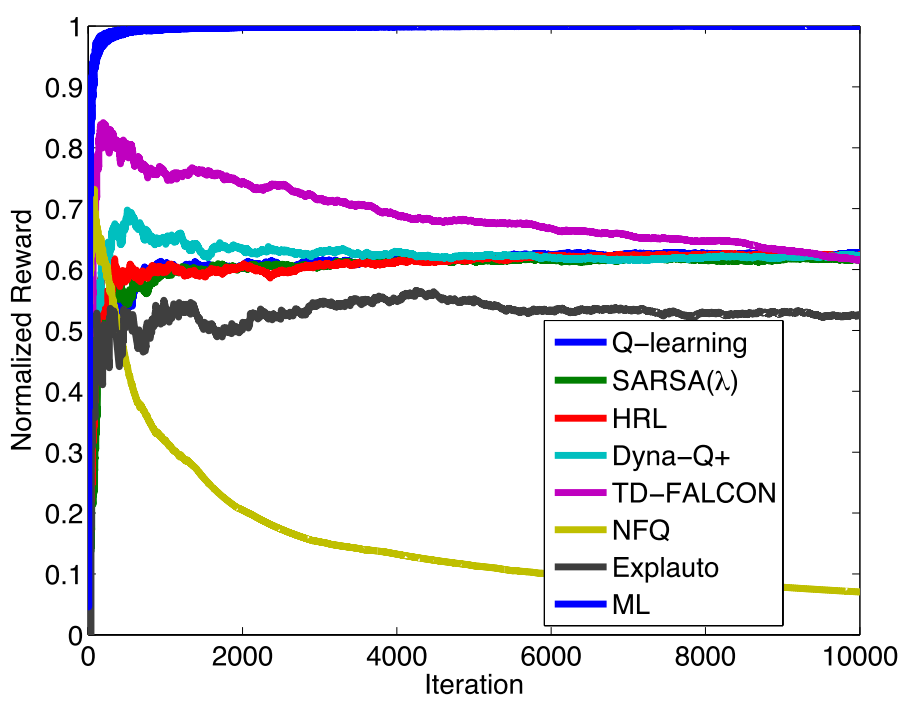
\includegraphics[width=0.55\linewidth]{rozdzial4/images/ml_vs_rl_blackbox_srate_1}
    \caption{Porównanie resultatów agenta ML z agentami RL dla $S_{rate}=1.0$. 
    Źródło: \cite{ml_vs_rl_comparative_study}.}
    \label{fig:ml_vs_rl_blackbox_srate1}
\end{figure}

Dla współczynnika $S_{rate}=1$ na początku większość agentów daje sobie radę 
porównywalnie tak samo. Sytuacja się zmienia już po około 500 iteracjach, 
gdzie wiele agentów przestaje sobie dawać radę w środowisku o coraz mniejszej
liczbie zasobów. Po około 2000 iteracjach większość agentów stabilizuje się
na tej samej wartości nagrody. Jedynym agentem, który daje sobie radę ze
zmnieniającym się otoczeniem jest agent z uczniem motywowanym. Wynika to
z najlepszego przystosowania do hierarchiczności świata tzn. zasobność 
surowców jest zależna od siebie hierarchicznie.  

Jeszcze bardziej zróżnicowane rezultaty i większe różnice pomiędzy agentem
z uczeniem motywowanym i agentem z uczeniem ze wzmocnieniem pojawiają
się dla współczynnika $S_{rate}=8.0$. Rezultaty widać na rysunku \ref{fig:ml_vs_rl_blackbox_srate8}.

\begin{figure}[h]
    \centering
    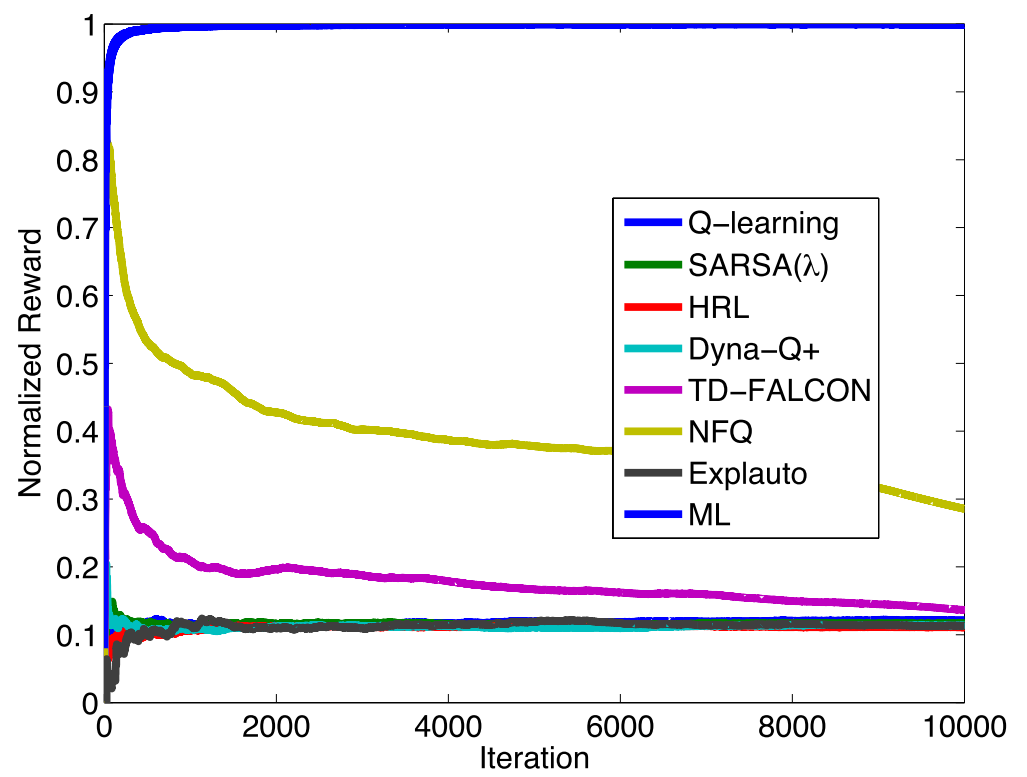
\includegraphics[width=0.6\linewidth]{rozdzial4/images/ml_vs_rl_blackbox_srate_8}
    \caption{Porównanie resultatów agenta ML z agentami RL dla $S_{rate}=8.0$. 
    Źródło: \cite{ml_vs_rl_comparative_study}.}
    \label{fig:ml_vs_rl_blackbox_srate8}
\end{figure}

Dla bardzo wrogiego środowiska, agent z uczeniem motywowanym daje sobie wciąż
radę, natomiast większość agentów z uczeniem ze wzmocnieniem, bardzo szybko 
stabilizuje się na niskiej wartości nagrody, ponieważ środowisko stało się
bardzo szybko wrogie poprzez niskie zasoby surowców. Agent z uczniem
motywowanym jest w stanie szybko stworzyć hierachię abstrokcyjnych bóli,
których obniżenie sprawia, że brakujące zasoby mogą zostać odbudowane.

